\documentclass{article}
\usepackage[spanish]{babel}
\usepackage{amsmath,graphicx}

%%%%%%%%%% Start TeXmacs macros
\newcommand{\tmaffiliation}[1]{\\ #1}
\newcommand{\tmem}[1]{{\em #1\/}}
\newcommand{\tmop}[1]{\ensuremath{\operatorname{#1}}}
%%%%%%%%%% End TeXmacs macros

\begin{document}

\title{Actividad 1}

\author{
  Jes{\'u}s mar{\'i}a Mora Mur
  \tmaffiliation{Universidad Internacional de La Rioja}
}

\date{2 noviembre 2026}

\maketitle

\section{Primer ejercicio}

El circuito que debemos analizar es el siguiente:

\begin{figure}[h]
  \raisebox{0.0\height}{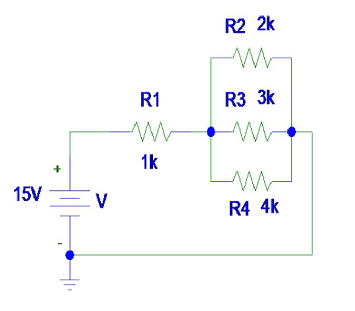
\includegraphics[width=5.95955496523678cm,height=5.22767447199265cm]{actividad1-1.pdf}}
  \caption{Circuito para analizar.}
\end{figure}

En primer lugar, debemos simplificar las resistencias del circuito para
conocer la intensidad que circula. Para las resistencias en paralelo, tenemos
que:
\[ R_{\tmop{eq}} = \frac{1}{\frac{1}{R_2} + \frac{1}{R_3} + \frac{1}{R_4}} =
   \frac{1}{\frac{1}{2000 \: \Omega} + \frac{1}{3000 \: \Omega} +
   \frac{1}{4000 \: \Omega}} = \frac{12000}{13} \: \Omega \approx 923.08 \:
   \Omega \]
Por otro lado, para la resistencia en serie con la que acabamos de calcular,
tenemos que:
\[ R_{\tmop{total}} = R_1 + R_{\tmop{eq}} = 1000 \: \Omega + \frac{12000}{13}
   \: \Omega = \frac{25000}{13} \: \Omega \]
Aplicando la {\tmem{Ley de Ohm}}, obtenemos la intensidad que circula por el
circuito:
\begin{equation}
  I_{\tmop{circuito}} = \frac{V}{R_{\tmop{total}}} = \frac{15 \: 
  \text{V}}{\frac{25000}{13} \: \Omega} = \frac{39}{5000} \:  \text{A} \approx
  7.8 \:  \text{mA}
\end{equation}
Con este dato, podemos obtener la ca{\'i}da de tensi{\'o}n en la primera
resistencia:
\[ V_1 = I \cdot R = \frac{39}{5000} \:  \text{A} \cdot 1000 \: \Omega =
   \frac{39}{5} \:  \text{V} \approx 7.8 \:  \text{V} \]
A las resistencias en paralelo entran:
\begin{eqnarray*}
  V = 7.2 \:  \text{V} &  & \\
  I = 7.8 \:  \text{mA} &  & 
\end{eqnarray*}
Al estar en paralelo, la tensi{\'o}n que pasa por las tres resistencias es
igual al voltaje entrante, estando la salida de las tres a $0 \:  \text{V}$.

\section{Segundo ejercicio}

La intensidad, a diferencia del voltaje se divide en funci{\'o}n de la
resistencia que hay en cada l{\'i}nea paralela. Esto es, seg{\'u}n la
{\tmem{Ley de Ohm}}:
\begin{equation}
  I = \frac{V}{R}
\end{equation}
Recordando que pasan $7.2 \:  \text{V}$, calculamos la intensidad:
\begin{eqnarray*}
  I_2 = \frac{7.2 \:  \text{V}}{2000 \: \Omega} = 3.6 \: \text{mA} &  & \\
  I_3 = \frac{7.2 \: \text{V}}{3000 \: \Omega} = 2.4 \: \text{mA} &  & \\
  I_4 = \frac{7.2 \: \text{V}}{4000 \: \Omega} = 1.8 \: \text{mA} &  & 
\end{eqnarray*}

\section{Tercer ejercicio}

Sabemos que la potencia disipada por una resistencia es:
\begin{equation}
  P = V \cdot I
\end{equation}
As{\'i}, calculamos la potencia para cada resistencia:
\begin{eqnarray*}
  P_1 = V_1 \cdot I_1 = 7.8 \: \text{V} \cdot 0.078 \: \text{A} \approx 0.61
  \: \text{W} &  & \\
  P_2 = V_2 \cdot I_2 = 7.2 \: \text{V} \cdot 0.036 \: \text{A} \approx 0.26
  \: \text{W} &  & \\
  P_3 = V_3 \cdot I_3 = 7.2 \: \text{V} \cdot 0.024 \: \text{A} \approx 0.17
  \: \text{W} &  & \\
  P_4 = V_3 \cdot I_3 = 7.2 \: \text{V} \cdot 0.018 \: \text{A} \approx 0.13
  \: \text{W} &  & 
\end{eqnarray*}
Sumando todas las potencias obtenemos la total del circuito:
\[ P_{\tmop{total}} = \Sigma^4_{n = 1} \: P_n = 1.17 \: \text{W} \]
que debe coincidir con la suministrada por la fuente:
\[ P_{\tmop{fuente}} = V_{\tmop{fuente}} \cdot I_{\tmop{fuente}} = 15 \:
   \text{V} \cdot 0.078 \: \text{A} = 1.17 \: \text{W} \]

\end{document}
